\section{Experimentation}
\label{sec:experimentation}

\subsection{Verification}

To confirm the model's basic operations, we ran it interactively with a wide
variety of values for every parameter. We verified, among other things, that
the CI2 mechanism does asymptote towards a fixed point as expected.
Figure~\ref{drifts_and_chases_asymptote} (left) depicts the average amount that each
agent's opinion was either ``pushed'' (or ``pulled'') towards an agent similar
enough (or dissimilar enough) on the comparison issue. These drift distances
decay over the course of about four hundred iterations until an equilibrium is
reached. Empirically, we discovered that an \textbf{openness} parameter value
of \textbf{.1}, and a \textbf{pushaway} of \textbf{.6}, worked well for
producing the CI2 effect.

\begin{figure}[ht]
\centering
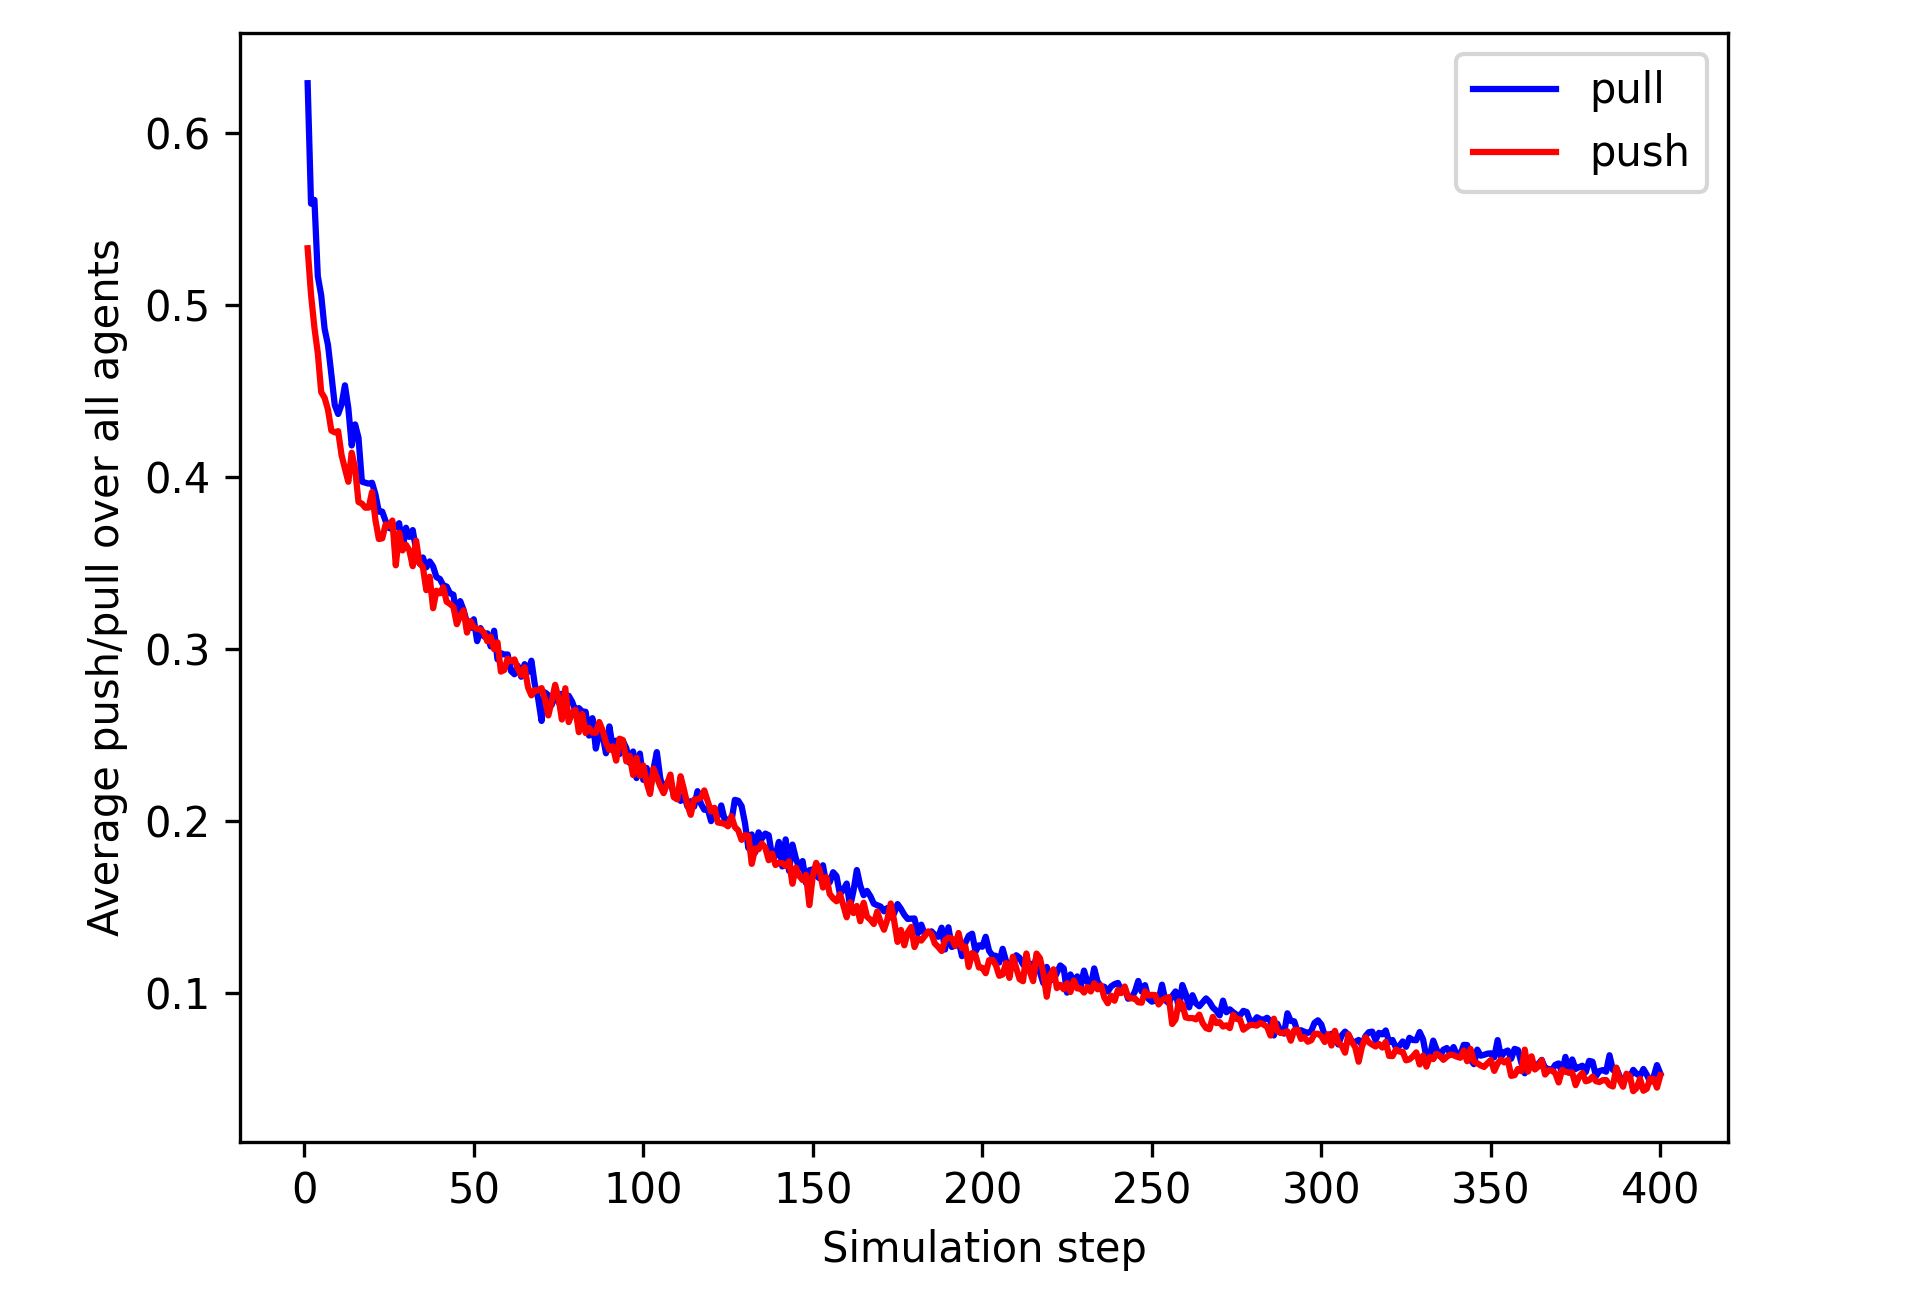
\includegraphics[width=0.45\textwidth]{assets/drifts_asymptote.png}
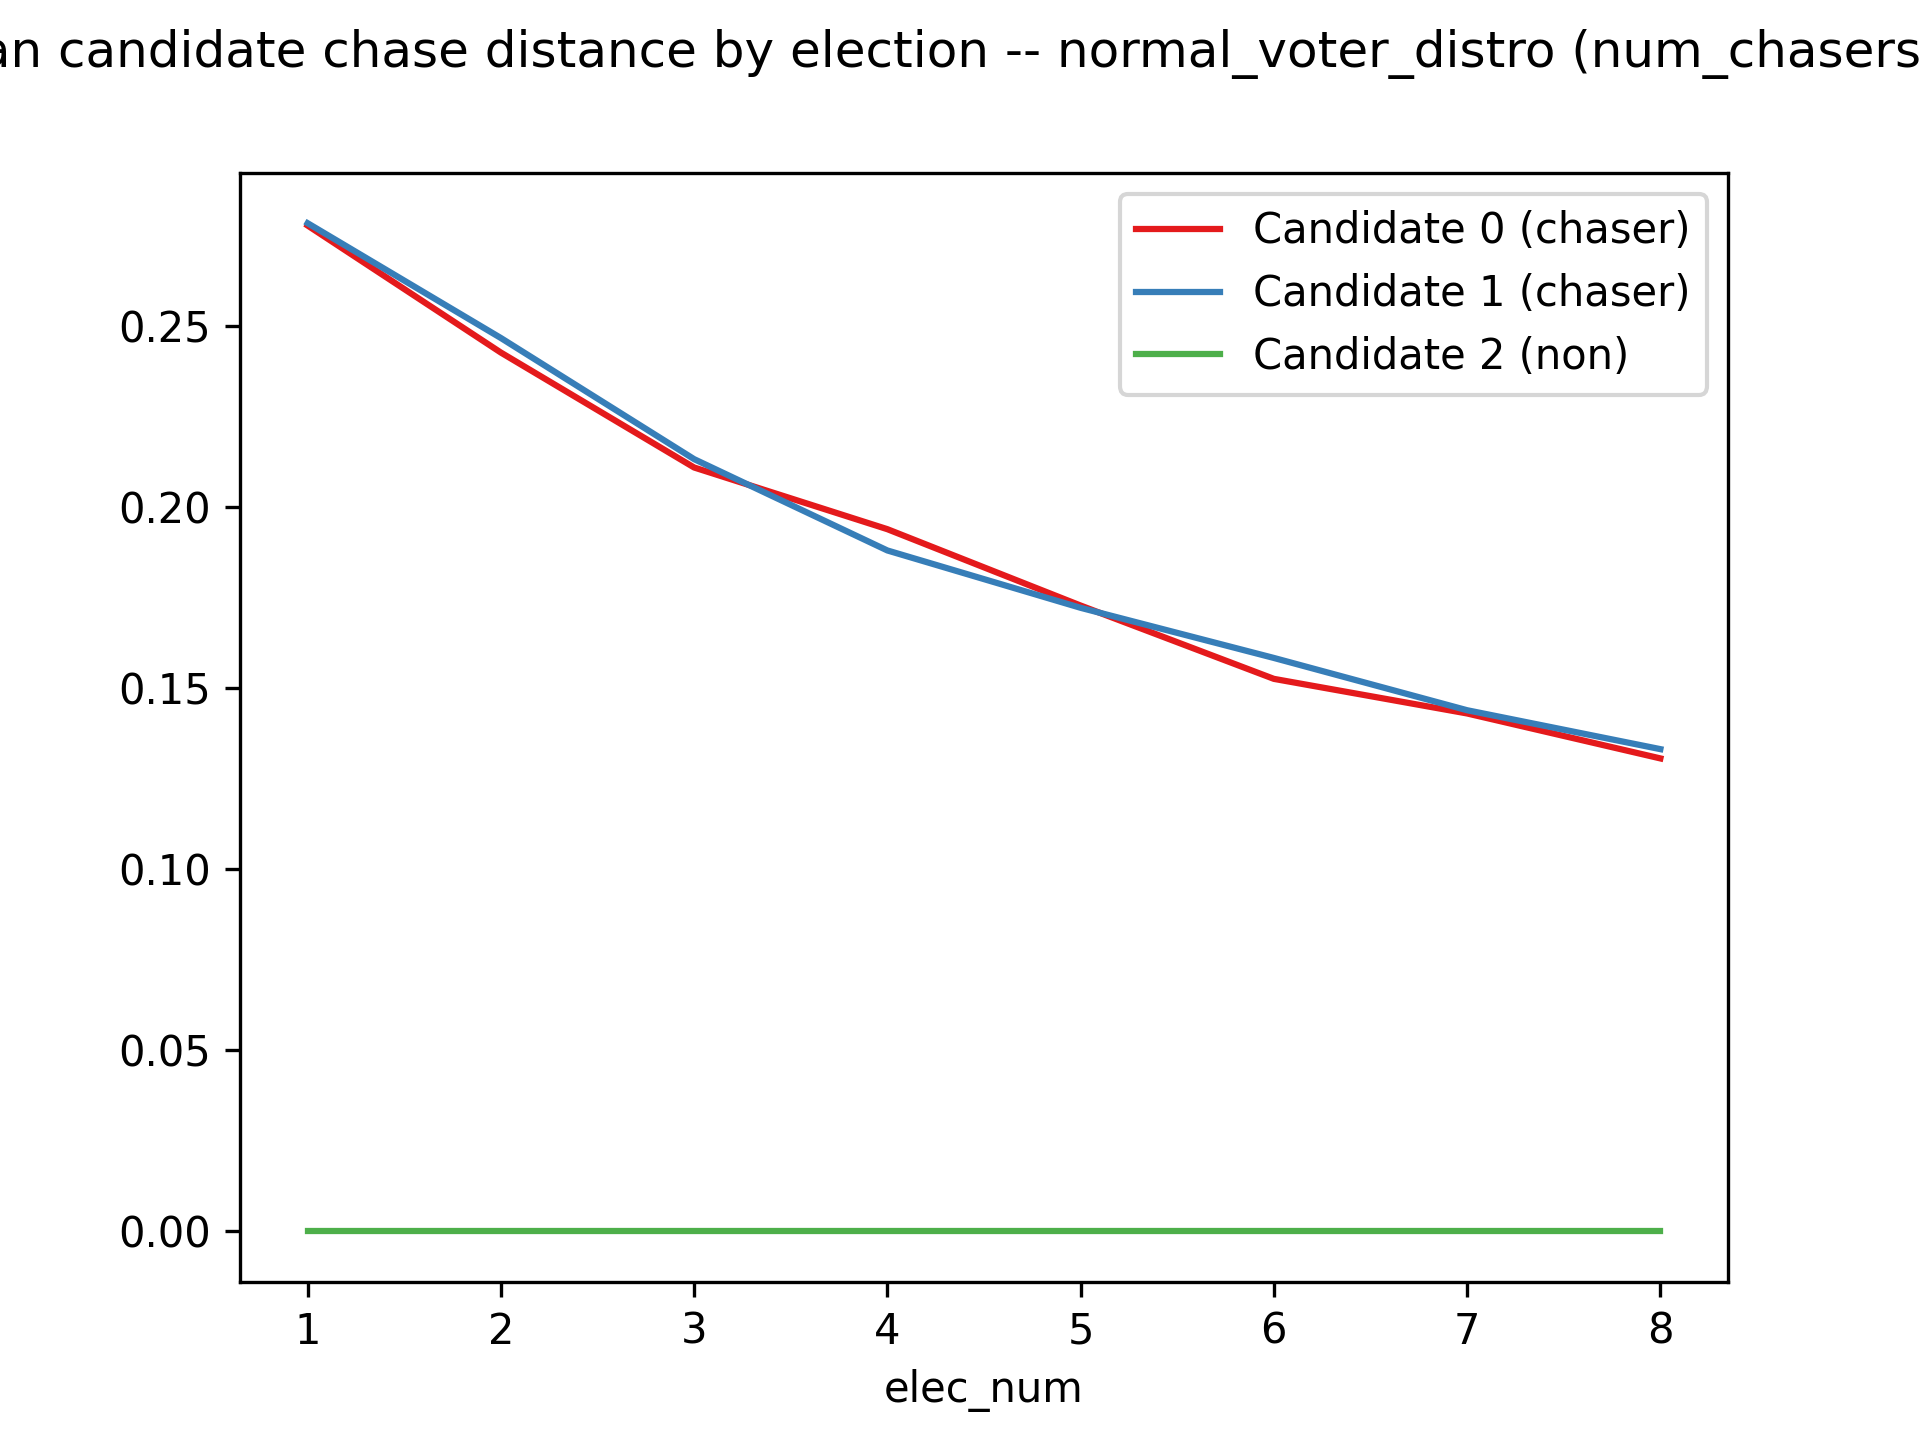
\includegraphics[width=0.45\textwidth]{assets/chase_dists_asymptote.png}
\caption{Both voters' drift movements (due to the CI2 mechanism approaching steady
state) and candidates' chase movements (due to all candidates reaching local
maxima in state space) asymptote to zero.}
\label{drifts_and_chases_asymptote}
\end{figure}

Similarly, as expected, the distances in opinion space that candidates
traversed in ``chasing'' voters also trend downward to zero. After reaping the
nearby ``low-hanging fruit'' (voters not locked in by any other candidate and
thus prime for poaching), candidates face diminishing returns when chasing any
further would jeopardize their existing voters. See
Figure~\ref{drifts_and_chases_asymptote} (right) for an illustration with two
chasing candidates.


\subsection{Independent variables}

%The model has a number of parameters that can be dialed, including: the
%openness and pushaway thresholds; the edge probability of the Erd

Two important independent variables center around the action choices of the two
kinds of agents. Candidates can be either chasers or non-chasers, and can alter
how far they are willing to move in opinion space in the pursuit of additional
voters. Voters adopt different voting algorithms, and thus the electorate can
be divided up into groups of varying sizes: for example, all rational; half
rational and half party; half party and one-fourth of each of the two Fast and
Frugal variants; and so on.

%- i.v.'s: SD focuses on candidate actions (i.e., how much they chase, etc.) and
%  HP focuses on voter actions (ie., the mix of algorithms)
%
%SD holds fixed: 1/3rd, 1/3rd, 1/6th, 1/6th
%    party switch thresh .2
%    openness .1
%    pushaway .6
%    edge probability .2
%
%HP holds fixed:
%    chase radius .2
%    num_chasers 3
%    num_candidates 3
%
%
%Both hold fixed:
%    num_opinions
%    N
%    
%- d.v.'s: one of us focuses on candidate winning, and the other focuses on
%  election rationality  


\subsection{Dependent variables}

% **(SD)**
% D.v.’s
%   Likelihood that election #n will turn out rational, for 1 <= n <= 8.
%   Candidate winning
%   Party switches
